\section{Barium Zirconate Structure}

Proton conducting oxides are of primary importance in the development of the next generation of solid oxide fuel cells. Interest in this category of electrolytes began with investigations carried out by Iwahara and associates \cite{Iwahara1981,Iwahara1988} in the 1980's. Their work demonstrated proton conduction by electrolysis of steam to show hydrogen gas formation on the opposite side of the cell. Many of the most promising materials that came under study in the following years are perovskites, which are ABO$_3$ ionic compounds where $A$ is a $2^+$ cation, $B$ is a $4^+$ cation and oxygen is in its usual $2^-$ oxidation state \cite{Uchida1983}. Perovskites remain among the most studied proton conducting materials and report the highest conductivities \cite{Kreuer2003}.

The perovskite structure falls within space group $Pm\bar{3}m$, with A-site cations on the corners of the unit cell, B-site cation at the center and oxygen at the face centers, as seen Figure \ref{back:fig:perovskite}. The stability of this structure of ions and the degree of distortion from the ideal cubic phases is frequently quantified by the simple calculation of the Goldschmidt tolerance factor 
\begin{equation}
    t = \frac{R_A + R_O}{\sqrt{2}(R_B + R_O)}
    \label{back:equ:goldschmidt}
\end{equation}
which is based on the ratio of the A-O and B-O distances given by the radii of A- and B- cations, $R_A$ and $R_B$ respectively, and the oxygen ion radius, $R_O$. The ideal cubic perovskite structure is given by a tolerance factor of $t=1$, while in practice cubic structure has been reported for $0.95 \leq t \leq 1.04$ \cite{SAMMELLS1992}. Tolerance factors from 0.70 to 0.90 reportedly result in an orthorhombic structure, while for tolerance factors greater than 1.05 result in sesquioxide structures \cite{Giaquinta1994}. K. S. Knight enumerated several distortion mechanisms that can occur in these perovskite structures including distortions or tilting of the BO$_6$ octahedra or displacements of the A- or B-site within their respective octahedra. These displacements can give rise to, for example, the ferroelectric behavior observed in BaTiO$_3$ \cite{Kwei1993}. Lattice distortions are further introduced by the presence of dopant ions, and the Goldschmidt tolerance factor is used as a measure of strain induced by these dopants relative to their undoped configuration. The effect of this distortion on the ionic conductivity will be discussed further after the mechanism of proton transport is introduced.


\begin{figure}
    \centering
    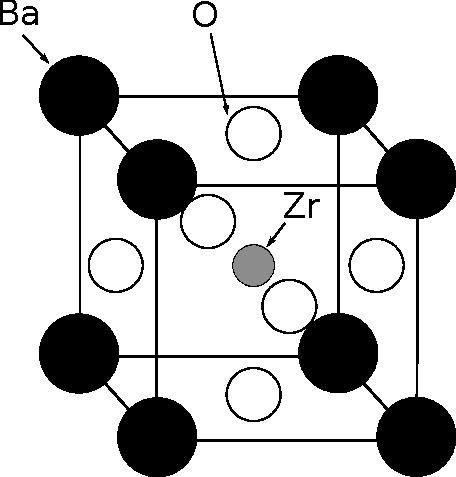
\includegraphics[width=.4\linewidth]{Figures/BaZrO_3-Zr-center.pdf}
    \caption[Cubic perovskite structure]{Cubic perovskite structure showing Zr centered view.}
    \label{back:fig:perovskite}
\end{figure}

\begin{table}
\centering
\caption{Goldschmidt tolerance factors of common perovskites. Radii stated in picometers.}
\label{back:table:goldschmidt}
\begin{tabular}{ llll }
\hline
 Compound & $R_A$ & $R_B$ & t \\
\hline
\hline
 BaZrO$_3$ & 149 & 86 & 0.917 \\
 BaCeO$_3$ & 149 & 101 & 0.857 \\
 SrCeO$_3$ & 132 & 101 & 0.804 \\
 BaTiO$_3$ & 149 & 74.5 & 0.970 \\
 SrZrO$_3$ & 132 & 86 & 0.861 \\
\hline
\end{tabular}
\end{table}

\begin{figure}
    \centering
    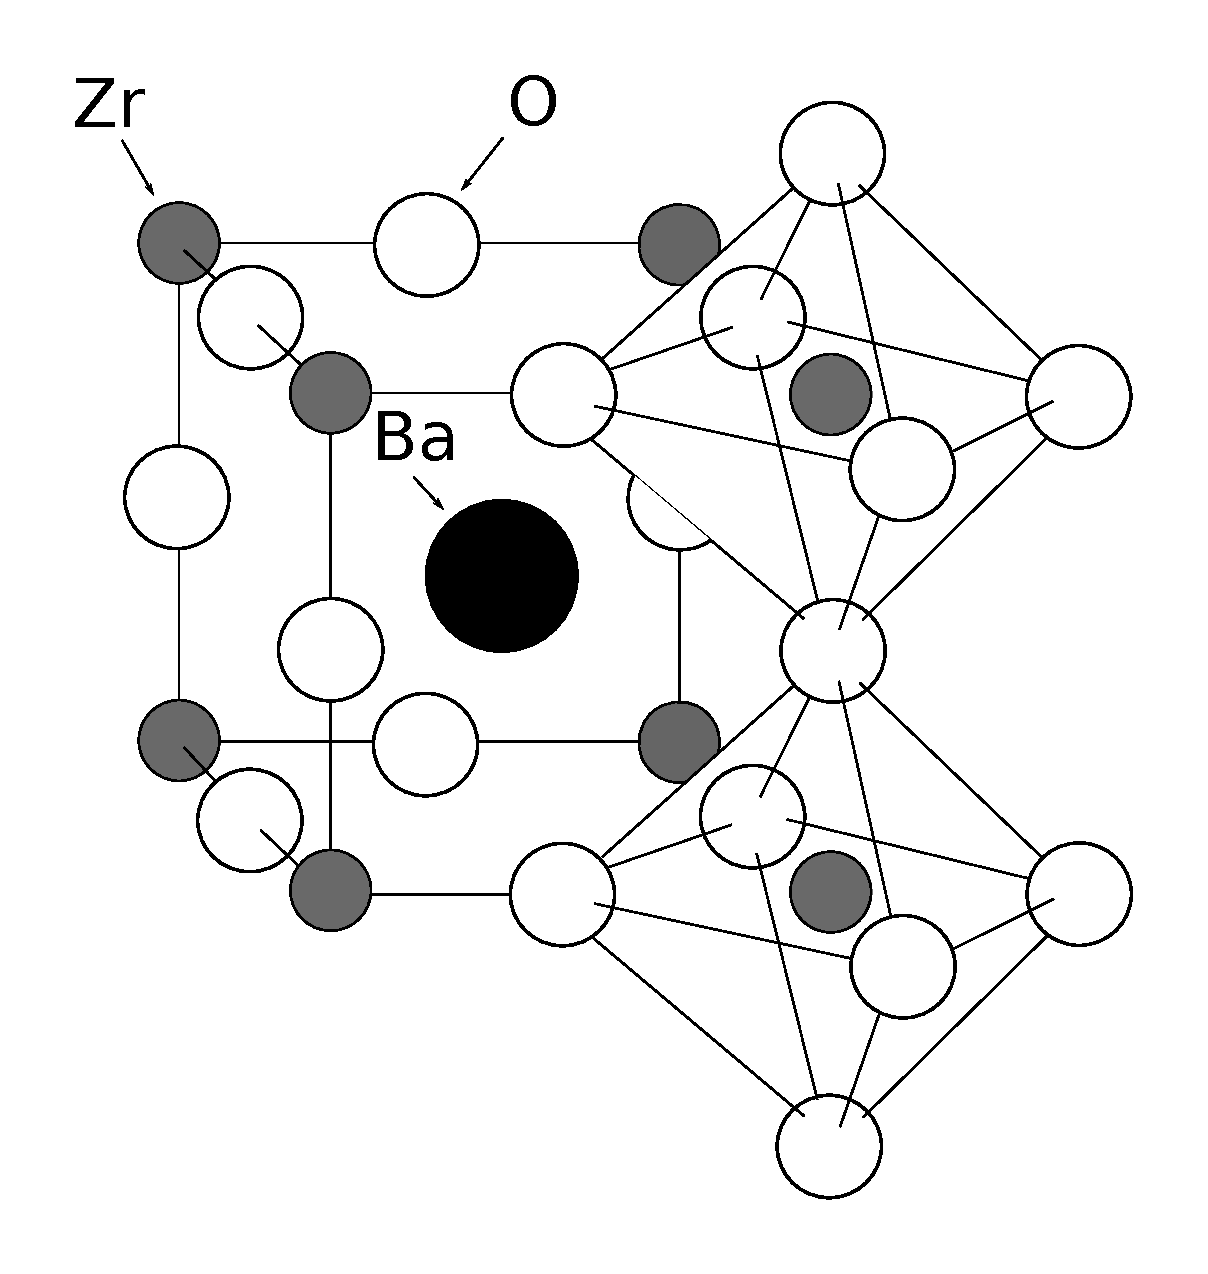
\includegraphics[width=.55\linewidth]{Figures/BaZrO_3-Zr-octahedra.pdf}
    \caption{Barium centered view of the barium zirconate structure showing ZrO$_6$ octahedra}
    \label{back:fig:octahedra}
\end{figure}

Strontium and barium based cerates were initially the class of perovskite most studied for high ionic conductivity. Barium cerate doped with gadolinium remains one of the highest proton conductors. But these cerates are vulnerable to decomposition in acidic gases such as CO$_2$ at elevated temperatures, forming alkaline earth carbonates according to the following reaction equation:
\begin{equation}
\mathrm{BaCeO_3 + CO_2 \rightarrow BaCO_3 + CeO_2}.
\end{equation}
This reaction is in fact a reversal of the most common high temperature solid state reaction synthesis method for these materials, as will be discussed in Chapter \ref{ch:bulk}. This precludes their use in fuel cells with carbon based fuels and thus interest in more chemically stable perovskites expanded to include the zirconates \cite{SCHOLTEN1993}. Therefore, the excellent chemical stability of barium zirconate under these conditions made its use in these applications more viable.